\documentclass[table, 12pt]{article}
\usepackage[T1]{fontenc}
\usepackage[utf8]{inputenc}
\usepackage[english]{babel}
\usepackage{graphicx}
\usepackage{titlesec}
\usepackage{hyperref}
\usepackage[usenames,dvipsnames]{xcolor}
\usepackage{float}
\usepackage[export]{adjustbox}
\usepackage{longtable}

\hyphenation{Te-lan-ga-na}
\hyphenation{an-a-lys-ing}
\hyphenation{a-gron-o-mists}
\hyphenation{a-gron-o-mist}
\titleformat{\paragraph}
{\normalfont\normalsize\bfseries}{\theparagraph}{1em}{}
\titlespacing*{\paragraph}
{0pt}{3.25ex plus 1ex minus .2ex}{1.5ex plus .2ex}


\begin{document}
\begin{titlepage}
    \centering
    {\scshape\large AY 2021/2022 \par}
    \vfill
    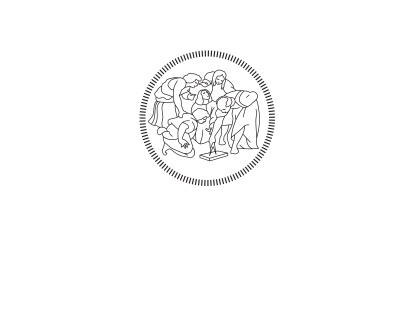
\includegraphics[width=100pt]{assets/logo-polimi-new}\par\vspace{1cm}
    {\scshape\LARGE Politecnico di Milano \par}
    \vspace{1.5cm}
    {\huge\bfseries DD\@: Design Document \par}
    \vspace{2cm}
    {\Large {Ottavia Belotti\quad Alessio Braccini\quad Riccardo Izzo}\par}
    \vfill
    {\large Professor\par
        Elisabetta \textsc{Di Nitto}}
    \vfill
    {\large \textbf{Version 1.0}\\ \today \par}
\end{titlepage}

\hypersetup{%
    pdfborder = {0 0 0}
}

\thispagestyle{plain}
\pagenumbering{gobble}
\mbox{}
\newpage
\pagenumbering{roman}
\tableofcontents
\newpage
\pagenumbering{arabic}

\section{Introduction}


\subsection{Purpose}
The purpose of this document is to provide a full technical description of the system described in the RASD document.
In this design document we discuss about both hardware and software architectures in terms of interaction among the components that represent the system.
Moreover there are mentions about the implementation, testing and integration process.
This document will include technical language so is primarily addressed to programmers but stakeholders are also invited to read it in order to understand the characteristics of the project.

\subsection{Scope}
The scope of this design document is to define the behavior of the system in both general and critical cases, and to design the architecture of the system by describing
logical allocation of the components and the interaction between them.
This document also extends in part to the implementation and testing plan, where one possible course of action is explained, user interface design of user applications and requirements traceability relating to the RASD.
\subsection{Definitions, acronyms, abbreviations}
\subsubsection*{Acronyms}
\begin{itemize}
    \item \textbf{DREAM}: \emph{Data-driven predictive farming}
    \item \textbf{RASD}: Requirement Analysis and Specification Document
    \item \textbf{DD}: Design Document
    \item \textbf{API}: Application Programming Interface
    \item \textbf{DBMS}: Database Management System
    \item \textbf{UML}: Unified Modeling Language
    \item \textbf{GPS}: Global Positioning System
    \item \textbf{IT}: Information Technology
    \item \textbf{GUI}: Graphic User Interface
\end{itemize}
\subsection{Revision history}

\subsection{Reference documents}
\begin{itemize}
    \item Specification document: "Assignment RDD AY 2021-2022"
    \item Requirements Analysis Specification Document (RASD)
    \item UML documentation: https://www.uml-diagrams.org/
    \item ArchiMate documentation: https://pubs.opengroup.org/architecture/archimate3-doc/
    \item Slides of the lectures
\end{itemize}
\subsection{Document structure}
\begin{itemize}
    \item \textbf{Section 1} gives a brief description of the design document, it describes the purpose and the scope of it including all the definitions, acronyms and abbreviations used. 
    \item \textbf{Section 2} delves deeply into the system architecture by providing a detailed description of the components, the interfaces and all the technical choices made for the development of the application.
    It also includes detailed sequence, component and ArchiMate diagrams that describes in depth the system.
    \item \textbf{Section 3} contains a complete description of the user interface, it includes all the client-side mockups with some graphs useful to understand the correct execution flow.
    \item \textbf{Section 4} links the RASD and the DD, it maps the goals and the requirements described in the RASD to the actual functionalities presented in this DD.
    \item \textbf{Section 5} presents a description of the implementation, testing and integration phases of the system components.
\end{itemize}
\section{Architectural Design}


\subsection{Overview}
\begin{center}
    \begin{figure}[H]
        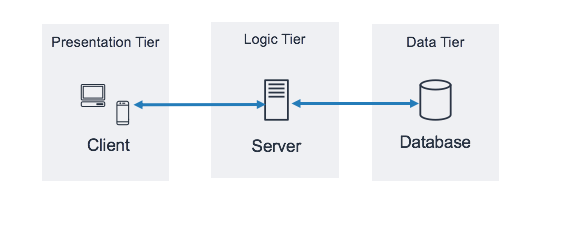
\includegraphics[scale=0.60, center]{assets/three-layer-architecture.png}
        \caption{Three-Layer Architecture}
        \label{fig: three-layer-architecture}
    \end{figure}
\end{center}

The system is a distributed application that follow the common client-server paradigm.
The architecture of the application is structured in three logic layers:
\begin{itemize}
    \item \textbf{Presentation Layer (P)}: it manages the presentation logic and handles the user actions.
    It is characterized by a GUI (Graphic User Interface) that allow the user to interact with the application in a simple and effective way.
    \item \textbf{Logic or Application Layer (A)}: it manages all the functionalities that has to be provided to the users, it is also responsible of data exchange between the client and the data sources.
    \item \textbf{Data Layer (D)}: it manages the access to data sources, it gets data from the database and move them through the other layers.
    It is essential to guarantee a high level of abstraction from the database in order to provide a model easy to use.
\end{itemize}

\begin{center}
    \begin{figure}[H]
        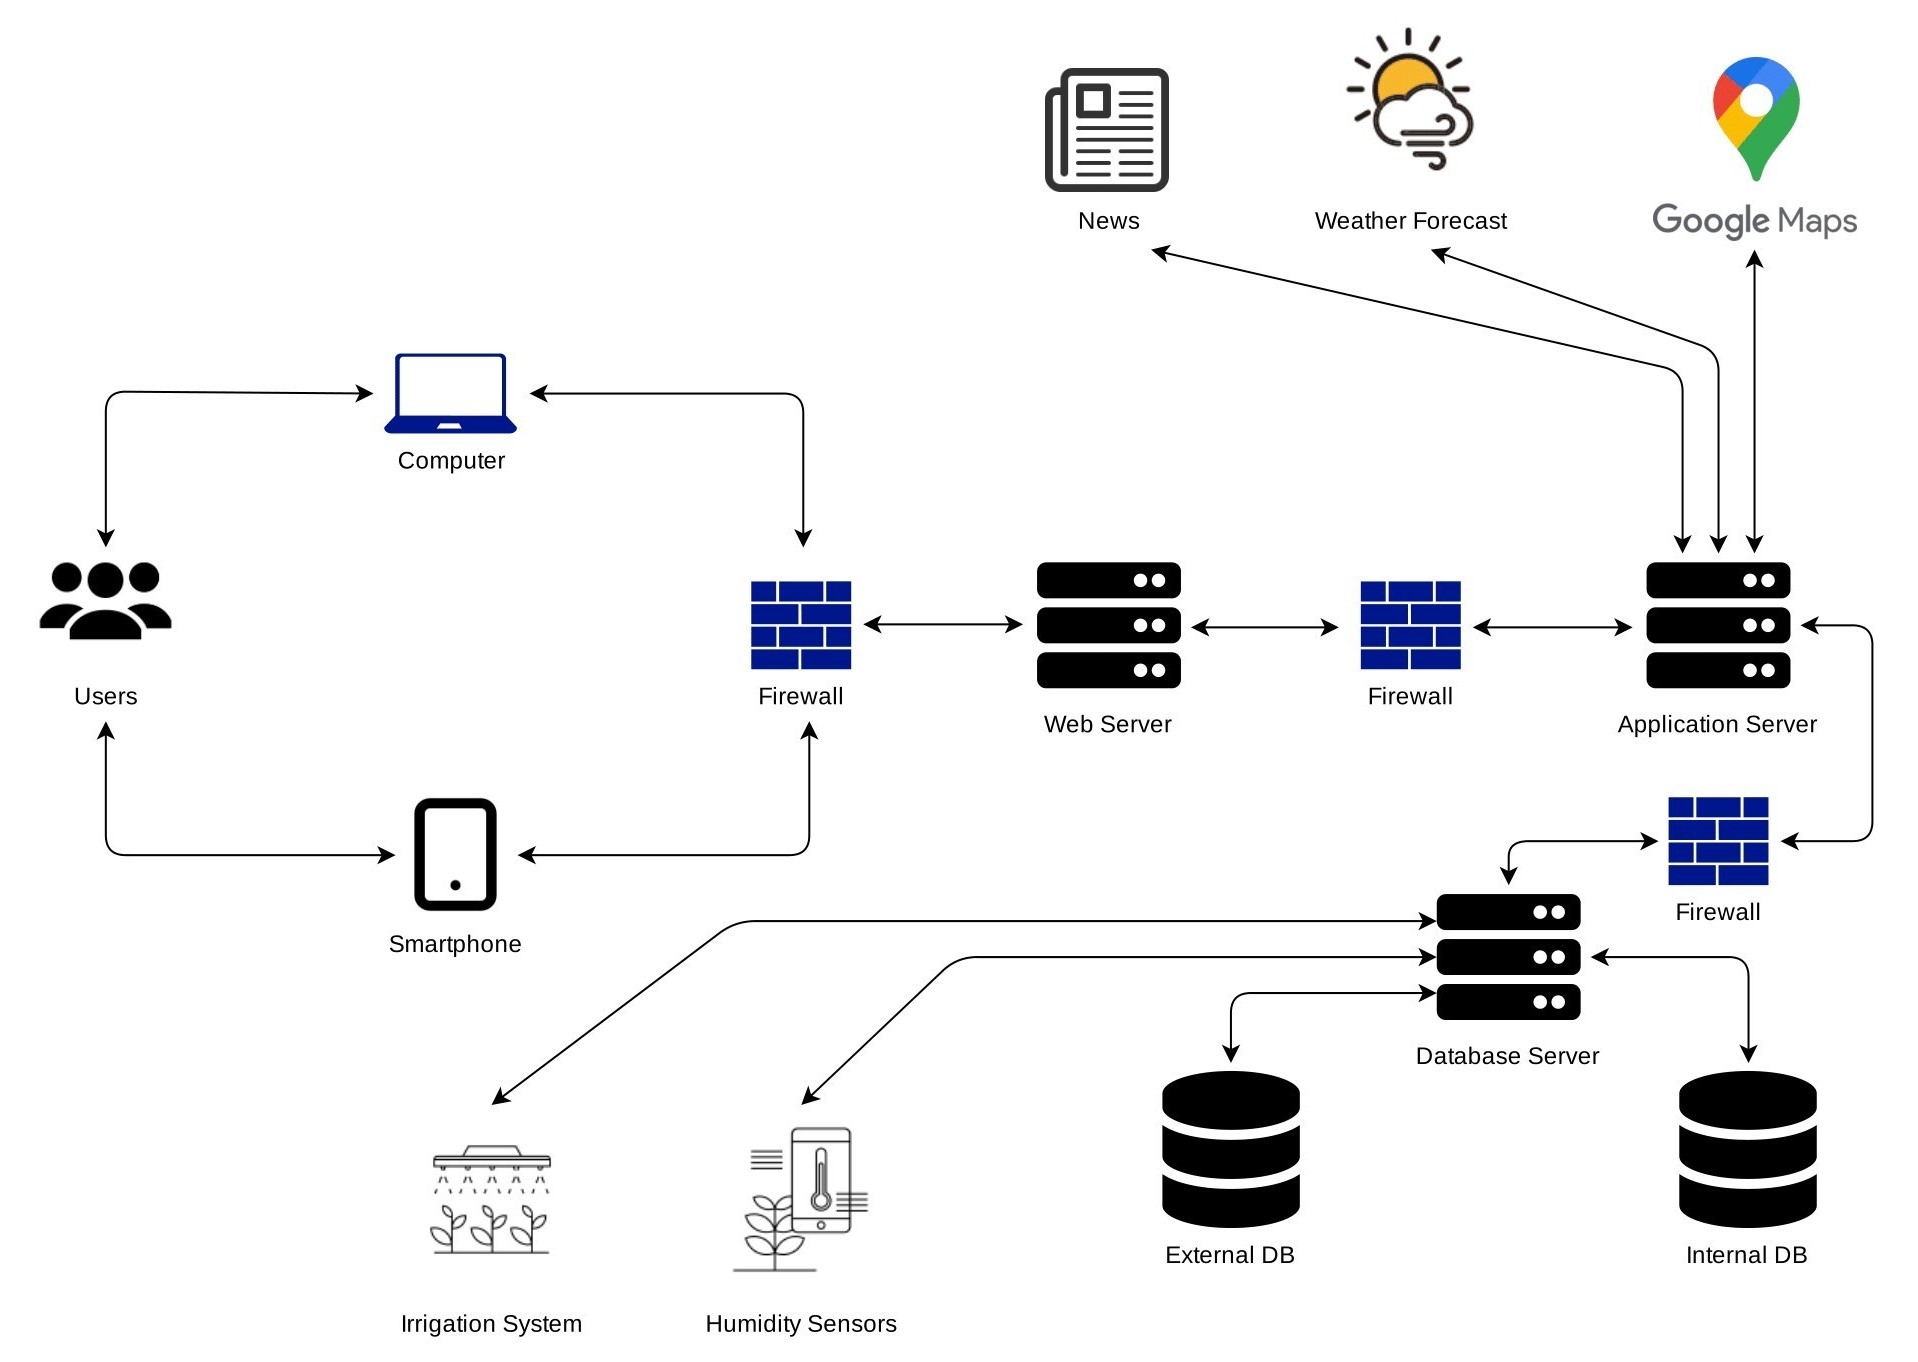
\includegraphics[scale=0.65, center]{assets/4-tier-architecture-scheme.jpg}
        \caption{High Level Architecture}
        \label{fig: high_level_architecture}
    \end{figure}
\end{center}

The system is based on a four-tier architecture(Client, Web Server, Application Server and Database Server), this ensures more flexibility and scalability.
The tiers are separated by firewalls in order to guarantee a higher level of security of the whole system.
A thin client is used to prevent heavy computation load client side, all the heavy operations are executed at the server side.
The client's devices can be a personal computer or a mobile device, both communicate directly with the application server through a web browser.
The application server communicates with the database server to store data.
For what concern the other components (water irrigation system, humidity sensors and weather forecasts system) they are connected to the web server that exchange data with the application server.
This allow to retrieve data like weather forecasts directly from it in order to show them to the user.
The web server also manages the data coming from the irrigation system and the humidity sensors.
Finally, to enable the geolocalization, the application server use the API provided by Open Street Map.
All the components will be described in depth in the following sections.

\subsection{Component view}
\subsubsection*{General Component View}
% don't panic: this is just the first draft of the general component
\begin{center}
    \begin{figure}[H]
        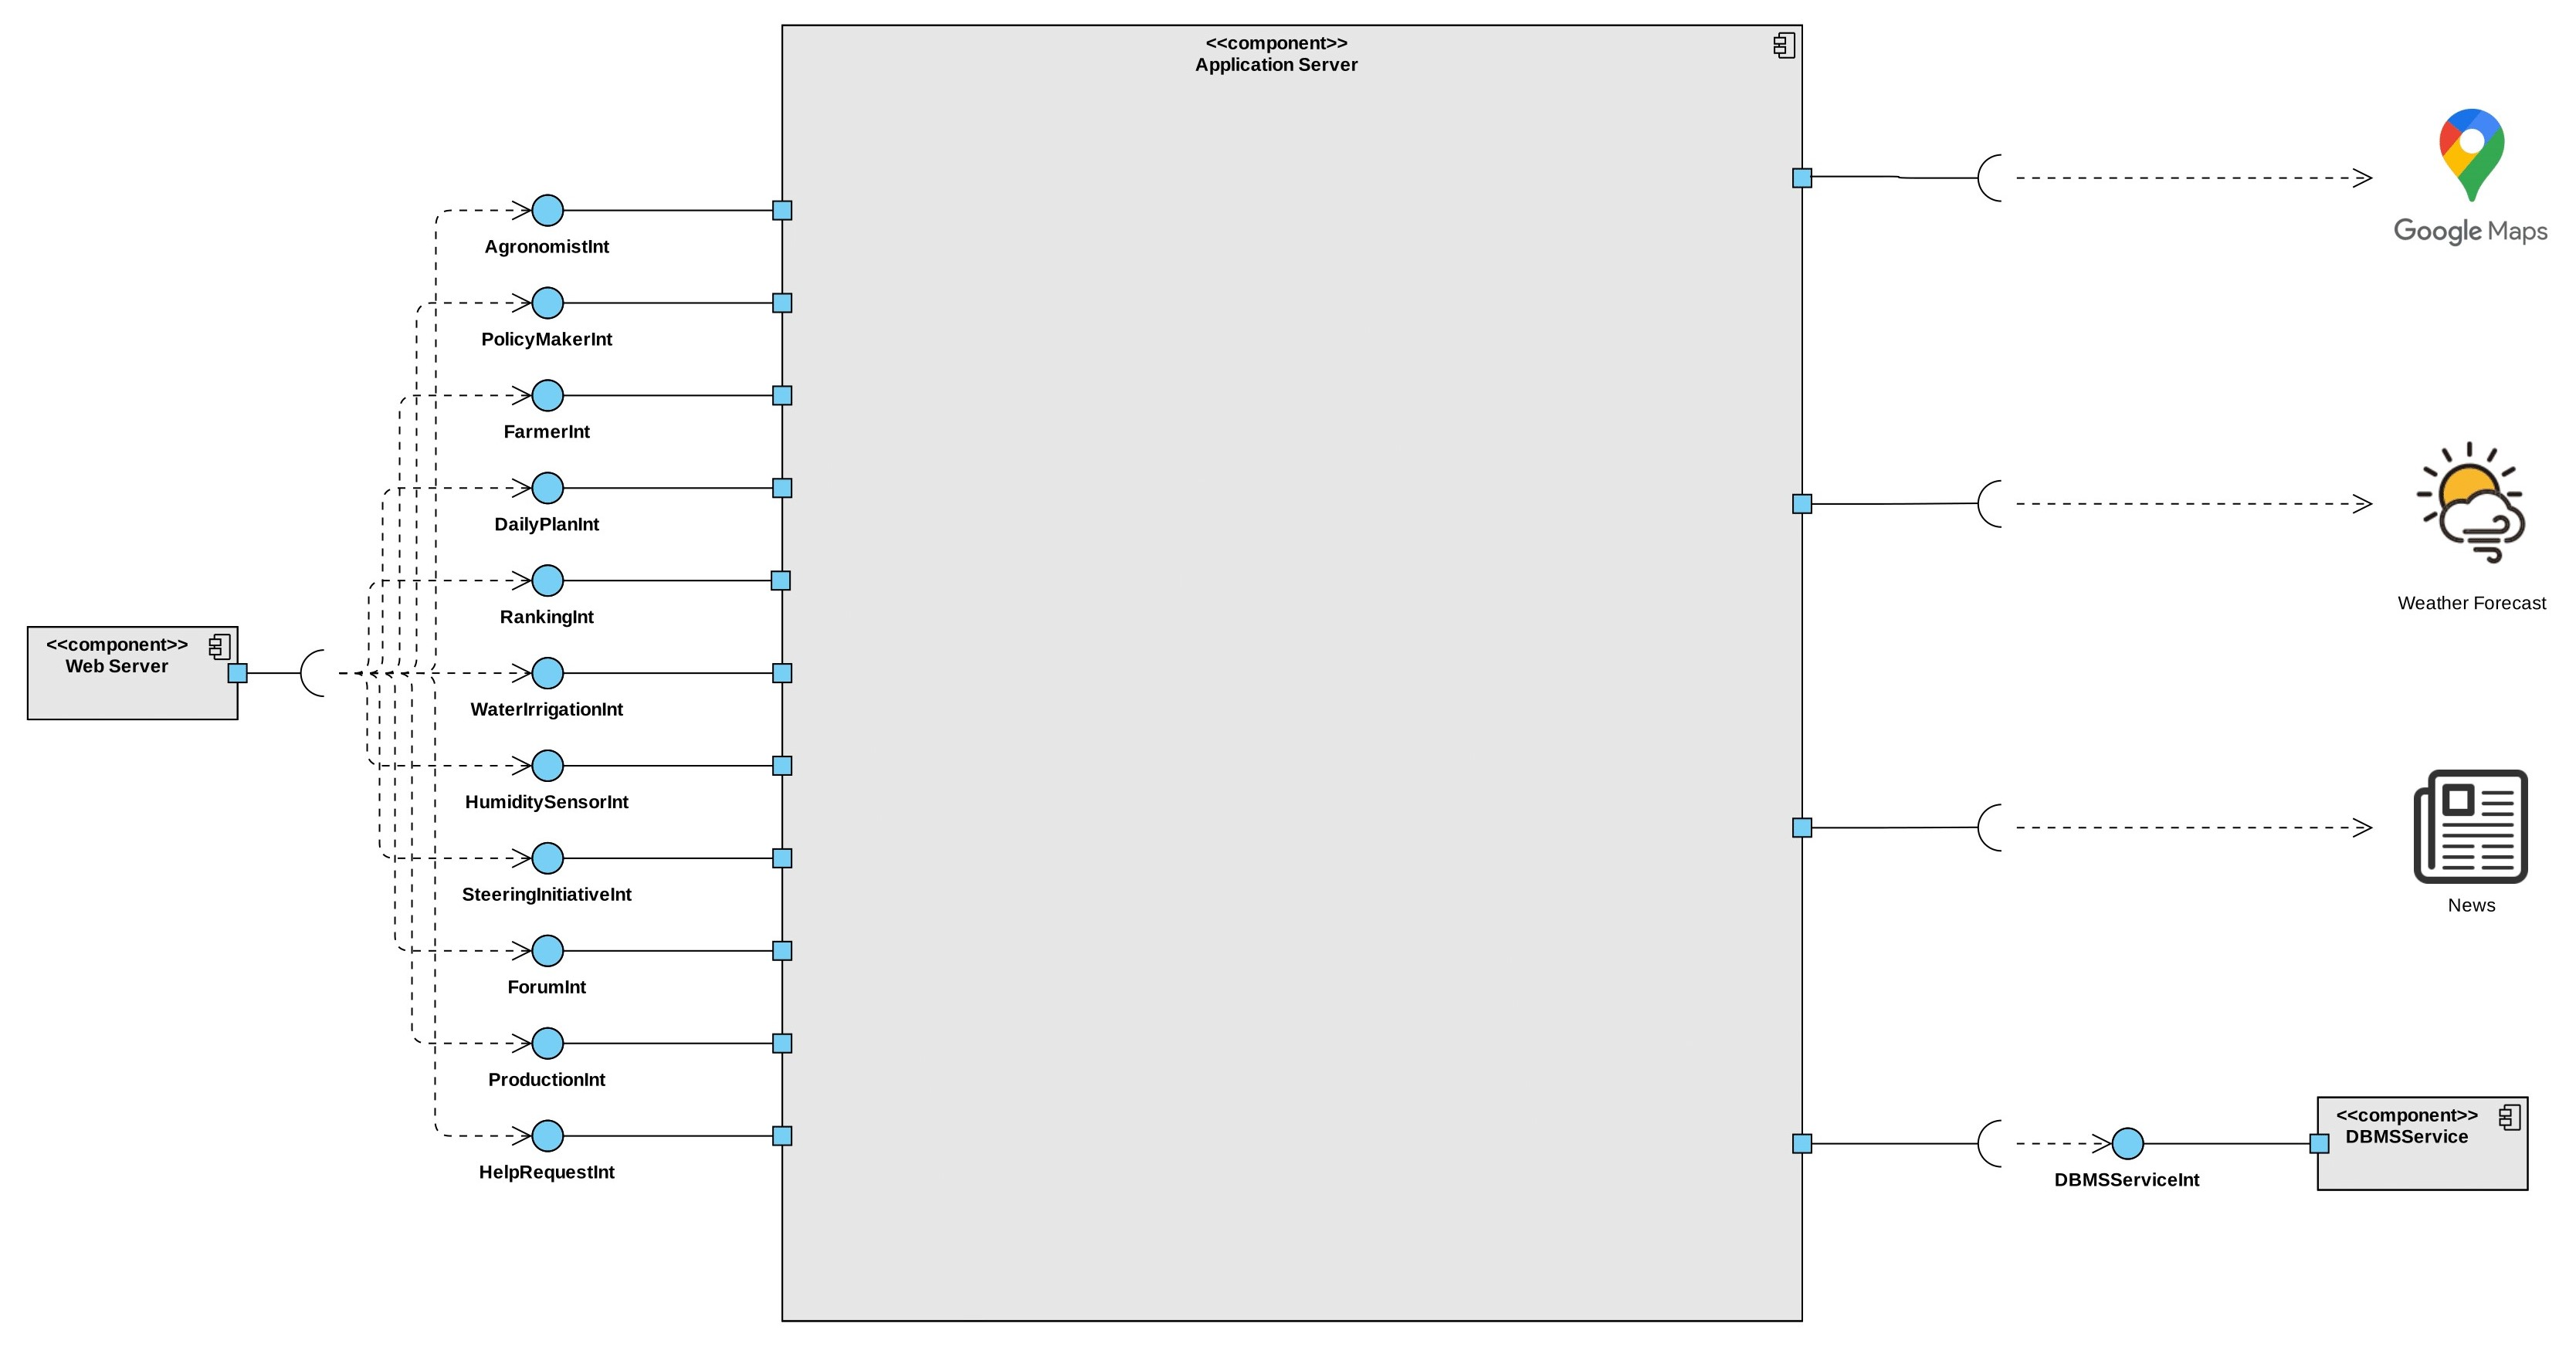
\includegraphics[scale=0.50, center]{assets/general-component-view.jpg}
        \caption{General Component View}
        \label{fig: general_component_view}
    \end{figure}
\end{center}

\subsubsection*{Application Server Component View}
% TODO: detailed component view 
\subsection{Deployment view}

\subsection{Runtime view}

\subsection{Component interfaces}

\subsection{Selected architectural styles and patterns}

\subsection{Other design decisions}

\section{User Interface Design}


\section{Requirements Traceability}


\section{Implementation, Integration and Test Plan}


\section{Effort Spent}


\section{References}


\end{document}